    \documentclass[10pt,a4paper]{article}

\usepackage{indentfirst}
%\usepackage{arev}
\usepackage{amsthm,amsfonts,amsmath,amssymb}
\usepackage[brazilian]{babel}
\usepackage[T1]{fontenc}
%\usepackage[latin1]{inputenc}
\usepackage[utf8]{inputenc}
%\usepackage{multicol}
\usepackage{setspace}
%\usepackage{natbib}
\usepackage[usenames,dvipsnames]{xcolor} 
\usepackage{pgf,tikz}
%\usepackage{algpseudocode}
\usepackage{float}
\usepackage{graphicx}
\usepackage{subfigure}
\usepackage{wrapfig}
%\usepackage{listings}
%\usepackage[linesnumbered, ruled, portuguese]{algorithm2e}
\usepackage{multirow}
%\usepackage{verbatim}
%\usepackage[active,tightpage]{preview}
%\PreviewEnvironment{tikzpicture}
%\setlength\PreviewBorder{5pt}
\usepackage{geometry}
\usepackage[pdftex]{hyperref}
\usepackage{listings}
\usepackage[normalem]{ulem}
\lstdefinelanguage{VHDL}{
  morekeywords=[1]{
abs,access,after,alias,all,and,architecture,array,assert,attribute,begin,block,body,buffer,bus,case
component,configuration,constant,disconnect,downto,else,elsif,end,entity,exit,file,for,function,generate,
generic,group,guarded,if,impure,in,inertial,inout,is,label,library,linkage,literal,loop,map,mod,
nand,new,next,nor,not,null,of,on,open,or,others,out,package,port,postponed,procedure,process,pure,
range,record,register,reject,return,rol,ror,select,severity,signal,shared,sla,sli,sra,srl,subtype,then,
to,transport,type,unaffected,units,until,use,variable,wait,when,while,with,xnor,xor,
ABS,ACCESS,AFTER,ALIAS,ALL,AND,ARCHITECTURE,ARRAY,ASSERT,ATTRIBUTE,BEGIN,BLOCK,BODY,BUFFER,BUS,CASE
COMPONENT,CONFIGURATION,CONSTANT,DISCONNECT,DOWNTO,ELSE,ELSIF,END,ENTITY,EXIT,FILE,FOR,FUNCTION,GENERATE,
GENERIC,GROUP,GUARDED,IF,IMPURE,IN,INERTIAL,INOUT,IS,LABEL,LIBRARY,LINKAGE,LITERAL,LOOP,MAP,MOD,
NAND,NEW,NEXT,NOR,NOT,NULL,OF,ON,OPEN,OR,OTHERS,OUT,PACKAGE,PORT,POSTPONED,PROCEDURE,PROCESS,PURE,
RANGE,RECORD,REGISTER,REJECT,RETURN,ROL,ROR,SELECT,SEVERITY,SIGNAL,SHARED,SLA,SLI,SRA,SRL,SUBTYPE,THEN,
TO,TRANSPORT,TYPE,UNAFFECTED,UNITS,UNTIL,USE,VARIABLE,WAIT,WHEN,WHILE,WITH,XNOR,XOR
  },
  morekeywords=[2]{
    STD_LOGIC_VECTOR,STD_LOGIC,IEEE,STD_LOGIC_1164,
    NUMERIC_STD,STD_LOGIC_ARITH,STD_LOGIC_UNSIGNED,std_logic_vector,
    std_logic
  },
  morecomment=[l]{--}
}

\colorlet{keyword}{blue!100!black!80}
\colorlet{STD}{Lavender}
\colorlet{comment}{green!80!black!90}
\lstdefinestyle{vhdl}{
  language     = VHDL,
  basicstyle   = \footnotesize \ttfamily,
  keywordstyle = [1]\color{keyword}\bfseries,
  keywordstyle = [2]\color{STD}\bfseries,
  commentstyle = \color{comment},
  breaklines=true,                % sets automatic line breaking
  tabsize=3                                % sets default tabsize to 2 spaces
}

\geometry{a4paper,inner=2.0cm,outer=2.0cm,top=2.0cm,bottom=2.0cm}


\newcommand{\pr}{\hspace*{0.6cm}}
\newcommand{\vesp}{\vspace*{.3cm}}

\newcommand{\sen}{\mbox{\,sen}}
\newcommand{\cotg}{\mbox{\,cotg\,}}
\newcommand{\tg}{\mbox{\,tg\,}}
\newcommand{\cose}{\mbox{\,cos\,}}
\newcommand{\expo}{\mbox{\,e\,}}
\newcommand{\logg}{\mbox{\,log}}
\newcommand{\Sum}{\displaystyle\sum}
\newcommand{\Prod}{\displaystyle\prod}
\newcommand{\Int}{\displaystyle\int}
\newcommand{\dint}{\, \mathrm{d}}
\newcommand{\Lim}{\displaystyle \lim}
\newcommand{\Frac}{\displaystyle\frac}

\newcommand{\Nc}{N_{cont}}
\newcommand{\Ni}{N_{int}}
\newcommand{\Ne}{N_{estrela}}

\newcommand{\Dparc}[2]{\dfrac{\partial #1}{\partial #2}}
\newcommand{\Dparcn}[3]{\dfrac{\partial^#3 #1}{\partial^#3 #2}}

\newcommand{\R}{\mathbb{R}}
\newcommand{\V}{\mathcal{V}}
\newcommand{\I}{I_u}
\newcommand{\Fi}{\varphi}
\newcommand{\se}{\mbox{ se }}
\newcommand{\norma}[1]{\left|\left| #1 \right|\right|}
\newcommand{\sistema}[1]{ \left\{ #1 \right. }

\newtheorem{exemplo}{\pr \sc Exemplo}[section]%[chapter]
\newtheorem{defi}{\pr \sc Defini\c{c}\~ao}[section]%[chapter]
\newtheorem{obs}{\pr \sc Observa\cao}[section]%[chapter]
\newtheorem{teor}{\pr \sc Teorema}[section]%[chapter]
\newtheorem{lema}{\pr \sc Lema}[section]%[chapter]
\newtheorem{prop}{\pr \sc Proposi\cao}[section]%[chapter]
\newtheorem{exercise}{\pr \sc Exerc\'\i cios}[section]%[chapter]
\newtheorem{alg}{\pr Algoritmo}[section]%[chapter]

\setlength{\columnsep}{1cm}

\setlength{\columnsep}{1cm}

\lstset{language=VHDL}

\lstdefinestyle{customc}{
  belowcaptionskip=1\baselineskip,
  breaklines=true,
  xleftmargin=\parindent,
  language=C,
  showstringspaces=false,
    keywordstyle=\bfseries\color{green!40!black},
  commentstyle=\itshape\color{purple!40!black},
  identifierstyle=\color{blue},
  stringstyle=\color{orange},
} 

%basicstyle=\footnotesize\ttfamily,

\lstset{escapechar=@,style=vhdl}

\begin{document}

\thispagestyle{empty}
\begin{center}
	UNIVERSIDADE DE SÃO PAULO – USP
	
	INSTITUTO DE CIÊNCIAS MATEMÁTICAS E DE COMPUTAÇÃO
	
	
	
	\vspace{7cm}
	
	\Large{\textbf{RELATÓRIO 2}}
	 
	\Large{\textbf{SME 104 – CÁLCULO NUMÉRICO}}
	
	\vspace{6cm}
	
	Alunos: Adams Vietro Codignotto da Silva - $6791943$ \\ Ana Clara Kandratavicius Ferreira - $7276877$
	
	\vspace{6cm}
	
	São Carlos
	
	2014
\end{center}
\section{Introdução}
O método de Euler é um método de primeira ordem usado para resolver PVIs, servindo de construção para o método a ser estudado neste trabalho: o Método de Euler Modificado. Esse método é explícito de ordem 2, com um erro de $O(h^3)$ por passo.\\
\section{Modelagem do Problema}
Como o método de Euler Modificado necessita que a EDO seja de primeira ordem, precisamos fazer com que o PVI, que é de ordem superior, seja reduzido para um sistema de equações de primeira ordem.\\
\subsection{Redução para Equação de Primeira Ordem}
Dado o PVI:
$$
\begin{cases}
y^{\prime\prime}=y+\textit{e}^x, x\in \quad [0,2]\\
y(0)=1\\
y^{\prime}(0)=0
\end{cases}
$$
Podemos usar uma mudança de variável, fazendo $y^{\prime}=z$, obtendo $z^{\prime}=y+\textit{e}^x$. Assim, a equação de segunda ordem fica reduzida ao sistema:
$$
\begin{cases}
y^{\prime}=z\\
z^{\prime}=y+\textit{e}^x, x\in \quad [0,2]\\
y(0)=1\\
z(0)=0
\end{cases}
$$
\subsection{Calculando os passos}
Para esse sistema, podemos utilizar a fórmula de Euler Modificado, uma vez que o mesmo é de primeira ordem, onde:
\begin{equation}
\nonumber
\begin{array}{ccc}
y_{n+1}&=&y_n+hf(x_n,y_n,z_n)\\
z_{n+1}&=&z_n+hg(x_n,y_n,z_n)
\end{array}
\end{equation}
Então, usando a fórmula acima, temos:
\begin{equation}
\nonumber
\begin{array}{ccc}
y_{n+1}&=&y_n+hz_n\\
z_{n+1}&=&z_n+h(y_n+e^{x_n})
\end{array}
\end{equation}
Fazendo n=0 e utilizando k=1 para $h_k=\frac{0.2}{2^k}$, obtemos:
\begin{equation}
\nonumber
\begin{cases}
y_1=y_0+h(z_0)=1+0.1(0)=1\\
z_1=z_0+h(y_0+e^{x_0})=0+0.1(1+\textit{e}^0)=0.2
\end{cases}
\end{equation}
\newpage
\section{Experimentos e Resultados}
\subsection*{i)}
O método foi testado para todos os valores de k definidos no enunciado do problema. Os resultados foram:
\begin{table}[H]
\centering
\begin{tabular}{|c|c|c|}     
\hline
     x &            y(x) &                 exata(x) \\ 
\hline  
  0.00 &        1.000000 &                 1.000000 \\ 
  0.05 &        1.002500 &                 1.002522 \\ 
  0.10 &        1.010131 &                 1.010179 \\ 
  0.15 &        1.023045 &                 1.023127 \\ 
  0.20 &        1.041418 &                 1.041539 \\ 
  0.25 &        1.065443 &                 1.065610 \\ 
  0.30 &        1.095338 &                 1.095557 \\ 
  0.35 &        1.131341 &                 1.131620 \\ 
  0.40 &        1.173715 &                 1.174061 \\ 
  0.45 &        1.222747 &                 1.223169 \\ 
  0.50 &        1.278752 &                 1.279259 \\ 
  0.55 &        1.342071 &                 1.342670 \\ 
  0.60 &        1.413071 &                 1.413774 \\ 
  0.65 &        1.492153 &                 1.492970 \\ 
  0.70 &        1.579748 &                 1.580691 \\ 
  0.75 &        1.676320 &                 1.677400 \\ 
  0.80 &        1.782368 &                 1.783598 \\ 
  0.85 &        1.898428 &                 1.899823 \\ 
  0.90 &        2.025075 &                 2.026649 \\ 
  0.95 &        2.162926 &                 2.164695 \\ 
  1.00 &        2.312639 &                 2.314621 \\ 
  1.05 &        2.474920 &                 2.477133 \\ 
  1.10 &        2.650522 &                 2.652986 \\ 
  1.15 &        2.840250 &                 2.842987 \\ 
  1.20 &        3.044964 &                 3.047995 \\ 
  1.25 &        3.265578 &                 3.268929 \\ 
  1.30 &        3.503069 &                 3.506766 \\ 
  1.35 &        3.758478 &                 3.762549 \\ 
  1.40 &        4.032912 &                 4.037388 \\ 
  1.45 &        4.327552 &                 4.332464 \\ 
  1.50 &        4.643652 &                 4.649037 \\ 
  1.55 &        4.982549 &                 4.988443 \\ 
  1.60 &        5.345663 &                 5.352106 \\ 
  1.65 &        5.734505 &                 5.741541 \\ 
  1.70 &        6.150681 &                 6.158355 \\ 
  1.75 &        6.595897 &                 6.604258 \\ 
  1.80 &        7.071967 &                 7.081069 \\ 
  1.85 &        7.580816 &                 7.590716 \\ 
  1.90 &        8.124492 &                 8.135250 \\ 
  1.95 &        8.705168 &                 8.716848 \\ 
  2.00 &        9.325149 &                 9.337822 \\ 
  \hline
\end{tabular}
\caption{Resultados para k=1}
\label{tab:1}
\end{table}
Podemos ver que pelos gráficos a solução obtida com o método de Euler Modificado ficou bem próxima da solução exata, mostrando até mesmo dificuldades em observar tal fato nos gráficos abaixo. O uso da tabela de erros acima foi necessário para que possamos visualizar com mais facilidade. A tabela para k=4, por ser muito extensiva, foi omitida deste relatório.

\begin{minipage}[b]{0.48\textwidth}
\centering
\begin{figure}[H]
\centering
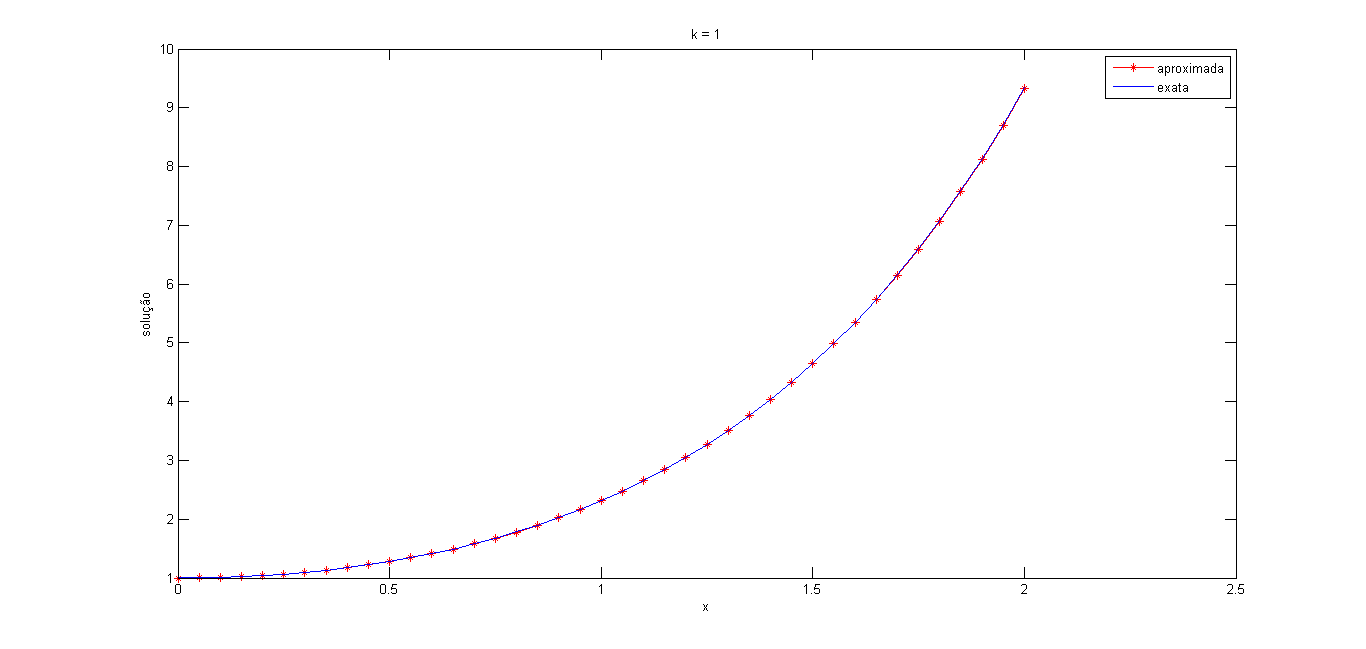
\includegraphics[scale=0.25]{k_1.png}
\caption{Erro para k=1}
\end{figure}
\end{minipage}
\begin{minipage}[b]{0.5\textwidth}
\centering
\begin{figure}[H]
\centering
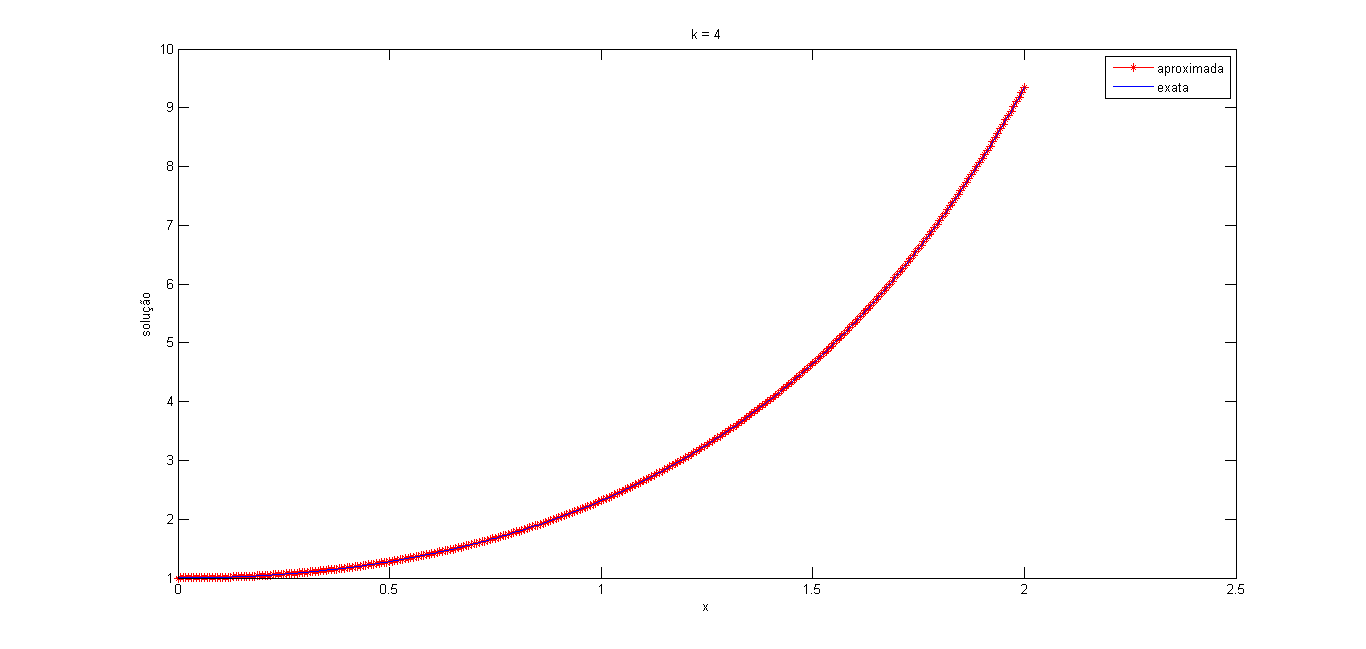
\includegraphics[scale=0.25]{k_4.png}
\caption{Erro para k=4}
\end{figure}
\end{minipage}
\subsection*{ii)}
Podemos notar que, com o aumento do número de passos (ou seja, com o aumento de k) o erro diminui:
\begin{figure}[H]
\centering
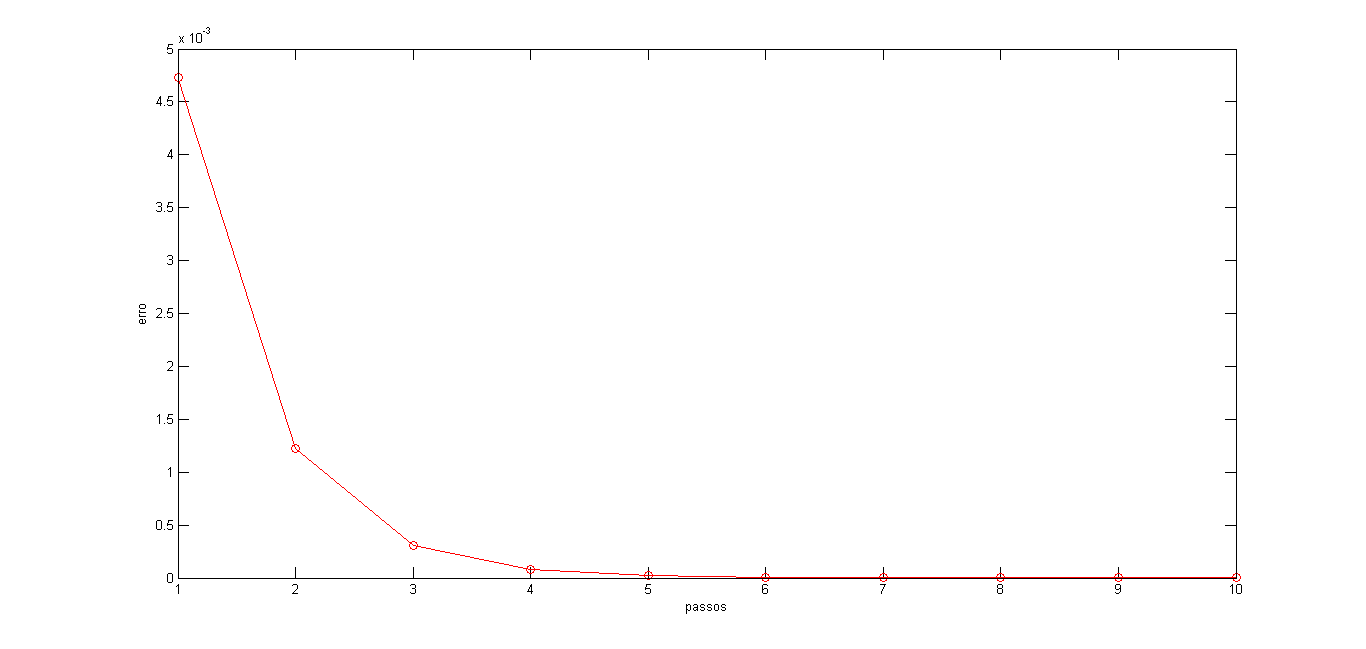
\includegraphics[scale=0.5]{err_plot.png}
\caption{Gráfico erro x passos}
\end{figure}
Com isso, podemos chegar à conclusão que a solução analítica está chegando cada vez mais próxima ao da solução exata, e para k=$\infty$, ou seja, quando h$\rightarrow$0, teremos a solução mais próxima da solução exata.

A tabela a seguir mostra a ordem de convergência calculada para o método implementado para resolver o PVI dado.

\begin{table}[H]
\centering
\begin{tabular}{|c|c|c|}   
\hline
\textbf{k}&\textbf{Ordem de convergência}\\ 
\hline
0&1.9007 \\
1&1.9520 \\
2&1.9765\\
3&1.9884\\
4&1.9942\\
5&1.9971\\
6&1.9986\\
7&1.9993\\
8&1.9996\\
\hline
\end{tabular}
\caption{Ordem de convergência do método Euler Modificado}
\label{tab:2}
\end{table}

\section{Conclusões}
Com os resultados obtidos neste trabalho, mostramos que a solução obtida é próxima à solução exata. Os erros obtidos mostram que o método se aproxima da solução exata com o aumento do número de passos, e que tal solução fica bem próxima à da exata com um passo próximo de 0. O método se mostrou extremamente fácil de se usar, uma vez determinado o PVI. Como mostrado na tabela \ref{tab:2}, foi possível observar que a ordem calculada está próxima à ordem esperada do método, que é de ordem 2.
 
\section{Implementação do Problema}
O método foi implementado utilizando a linguagem Matlab, e todas as funções utilizadas para o mesmo estão abaixo.\\
O programa é designado para exibir a ordem de convergência do método de Euler Modificado ao resolver o PVI do enunciado, podendo ser facilmente modificado para exibir a solução exata do mesmo. A única entrada do programa é o valor de k, determinando a quantidade de passos.
\newpage
\begin{verbatim}
%Calcula solucao de um PVI dado um k
%retorna a ordem de convergencia

function y2 = Euler(k)
[erro1,Y1,Exata1] = Euler_Modificado(k);
[erro2,Y2,Exata2] = Euler_Modificado(k+1);
y2 = OrdemEuler(erro1,erro2);
end

function [erro,YY,VExata]=Euler_Modificado(k)
h=0.2/(2^k);                        %m varia de 1 a 4
intervalo=[0,2];                    %define o intervalo de x
a=intervalo(1);
b=intervalo(2);
passos=(b-a)/h;                     %define número de passos
VErro=zeros(passos,1);              %vetor de erro para calculo da norma2
x=intervalo(1);                     %pega x inicial
y=[1;0];                            %define matrix de y(0) e y'(0)
VExata=zeros(passos,1);             %vetor de valores da solucao exata
YY=zeros(passos,1);
VExata(1)=Exata(x);                     %inicializa primeira posicao da solucao exata
VErro(1)=y(1)-Exata(x);
YY(1)=y(1);
% fileID = fopen('exp.txt','w');                %todas as operacoes de file são para exibir a saida de todos os pontos
                                                %no modo x|y(x)|exata(x) em um arquivo chamado exp.txt
% fprintf(fileID,'\\begin{tabular}{|c|c|c|}');
% fprintf(fileID,'%6s & %15s & %24s \\\\ \n','x','y(x)','exata(x)');
% fprintf(fileID,'\\hline');
% fprintf(fileID,'%6.2f & %15.6f & %24.6f \\\\ \n',x,y(1),Exata(x));
for i=1:passos
    k1=F(x,y);                      %k1 e k2 também são vetores
    k2=F(x+h/2,y+(h*(k1/2)));
    y=y+(h*k2);                     %calcula a matrix y(x) e y'(x)
    x=x+h;                          %avanca o ponto
    VErro(i+1)=y(1)-Exata(x);         %para calcular a norma2
    VExata(i+1)=Exata(x);             %para calcular a norma2
    YY(i+1)=y(1);

%     fprintf(fileID,'%6.2f & %15.6f & %24.6f \\\\ \n',x,y(1),Exata(x));
end
% fprintf(fileID,'\\end{tabular}');
% fclose(fileID);
erro = norm(VErro,2)/norm(VExata,2);%calcula erro do método em relacao à solucao exata
end

function t = F(x,y)
t=[y(2);y(1)+exp(x)];               %definindo a F(x,y)
end

function result = Exata(x)          %formula da solucao exata
result = ((exp(x)*(1+2*x))+3*exp(-x))/4;
end

function ordem = OrdemEuler(erro1, erro2)
ordem = log(erro1/erro2)/log(2);    %calculo da ordem de convergencia
end
\end{verbatim} \color{black}
\end{document}
